%%%%%%%%%%%%%%%%%%%%%%%%%%%%%%%%%%%%%%%%%%%%%%%%%%%%%%%%%%%%%%%%%
%%                                                       GLOSSARY
%%%%%%%%%%%%%%%%%%%%%%%%%%%%%%%%%%%%%%%%%%%%%%%%%%%%%%%%%%%%%%%%%

\ifPrintGlossary
    \setglossarystyle{list}
    \printglossaries
\fi

%%%%%%%%%%%%%%%%%%%%%%%%%%%%%%%%%%%%%%%%%%%%%%%%%%%%%%%%%%%%%%%%%
%%                                                  BIBLIOGRAPHY
%%%%%%%%%%%%%%%%%%%%%%%%%%%%%%%%%%%%%%%%%%%%%%%%%%%%%%%%%%%%%%%%%

\clearpage
\phantomsection
\addcontentsline{toc}{chapter}{Bibliography}

% TODO: improve bibtex settings, maybe move to biblatex. Currently invoking bibtex via the command
%       line, but want to change some settings. (E.g., include URL and DOI hyperlinks.)
% See https://tex.stackexchange.com/questions/3587/how-can-i-use-bibtex-to-cite-a-web-page
\bibliographystyle{\Bibstyle}
\ifx\Bibsettings\empty
    \bibliography{\Bibsettings,Thesis}
\else
    \bibliography{Thesis}
\fi

%%%%%%%%%%%%%%%%%%%%%%%%%%%%%%%%%%%%%%%%%%%%%%%%%%%%%%%%%%%%%%%%%
%%                                              CURRICULUM VITAE
%%%%%%%%%%%%%%%%%%%%%%%%%%%%%%%%%%%%%%%%%%%%%%%%%%%%%%%%%%%%%%%%%

\ifHasCurriculumVitae
    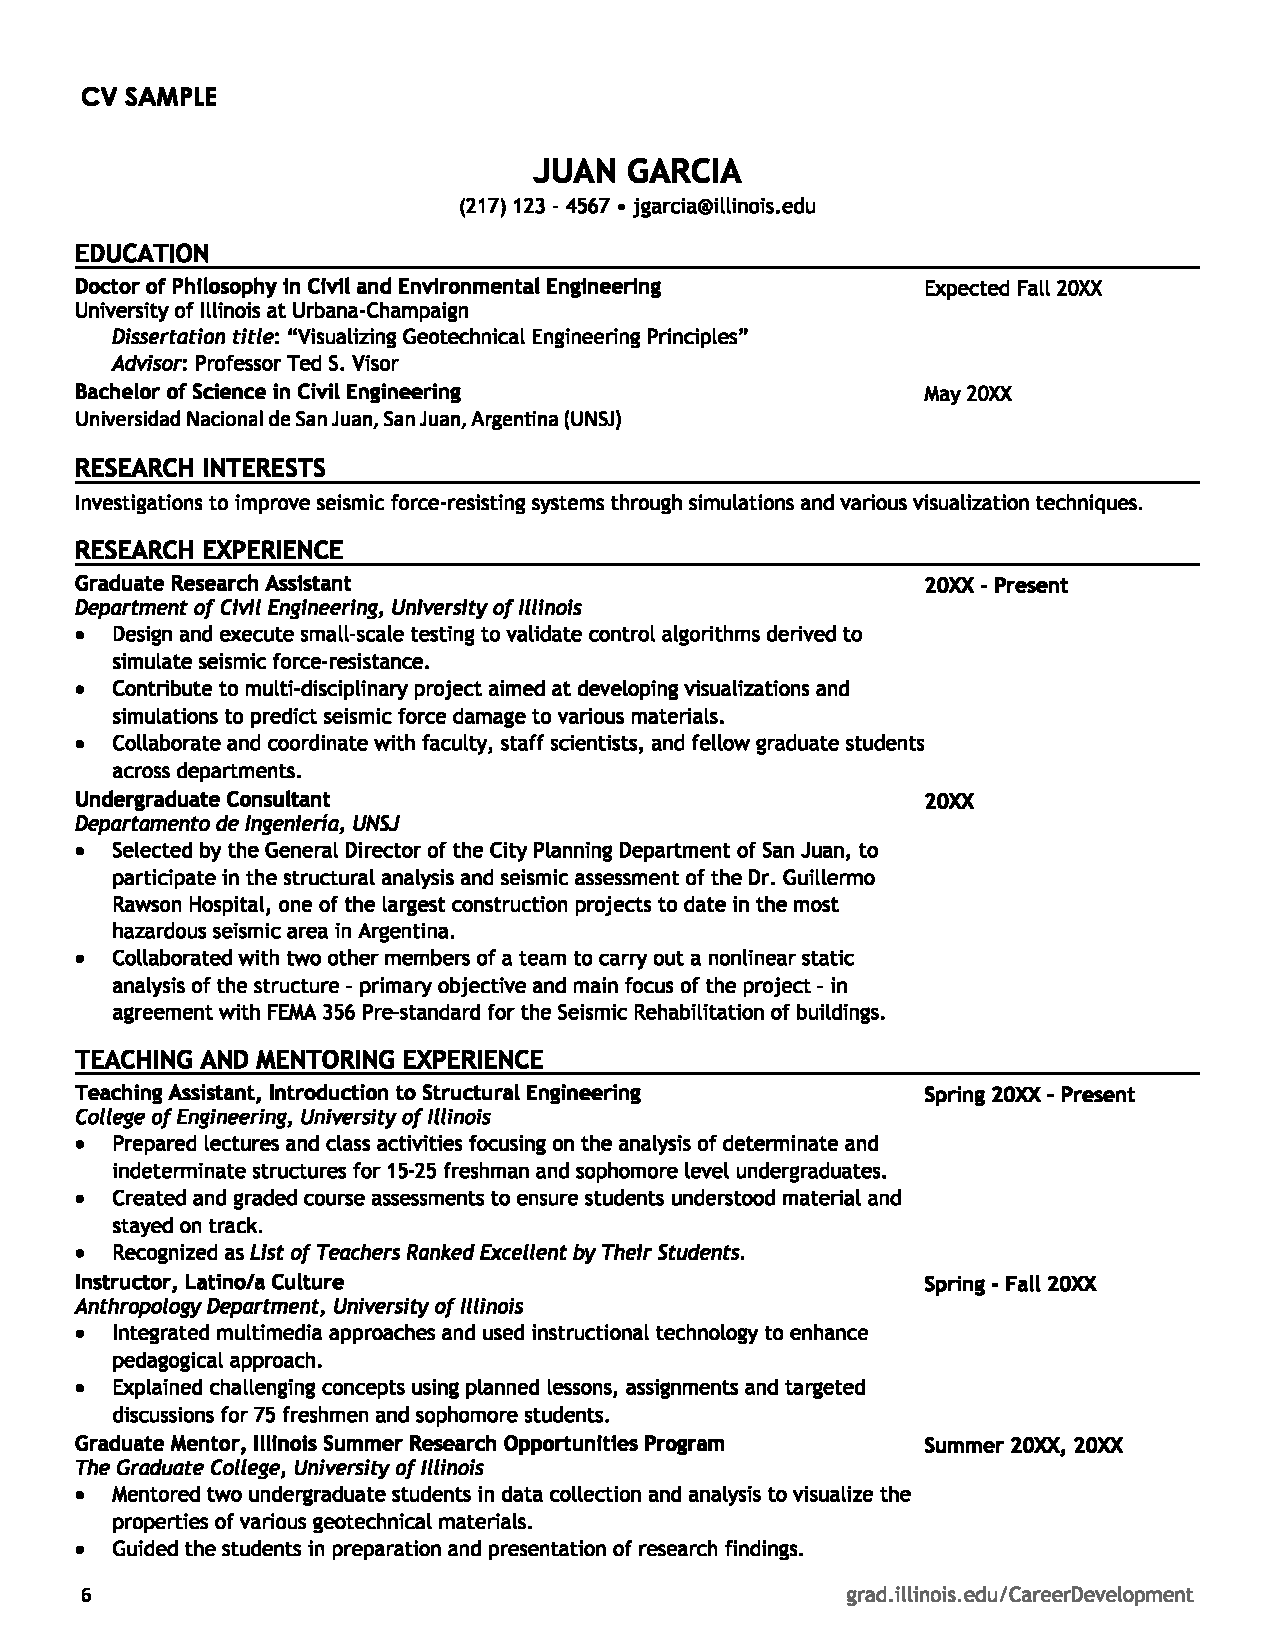
\includepdf[pages=-,pagecommand={\thispagestyle{plain}}]{Forms/CurriculumVitae.pdf}
\fi

%%%%%%%%%%%%%%%%%%%%%%%%%%%%%%%%%%%%%%%%%%%%%%%%%%%%%%%%%%%%%%%%%
%%                                        SCHOLARWORKS AGREEMENT
%%%%%%%%%%%%%%%%%%%%%%%%%%%%%%%%%%%%%%%%%%%%%%%%%%%%%%%%%%%%%%%%%

\ifIncludeForms
    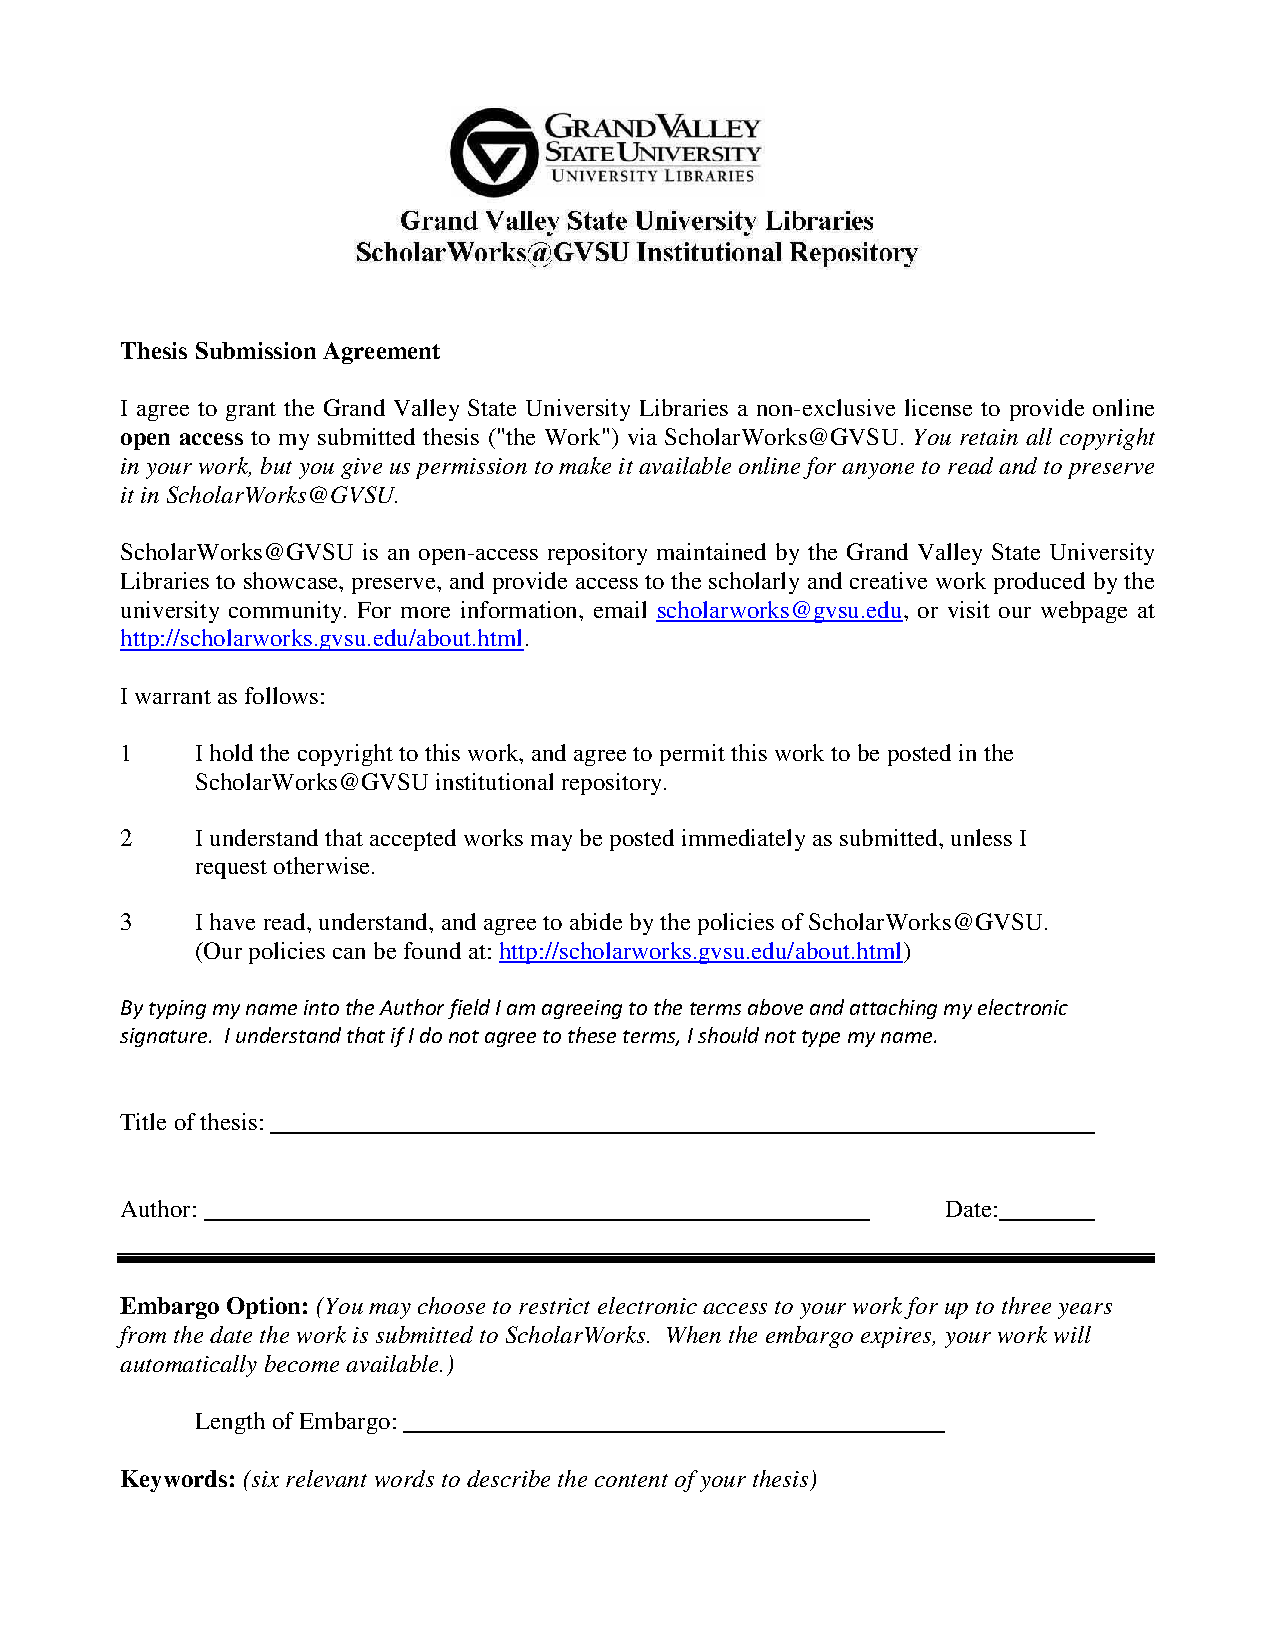
\includepdf{Forms/ScholarWorksAgreement.pdf}
\fi
